\section{Mjukvaruarkitektur}

Arkitekturen designades utgående samma principer som den tekniska arkitekturen, systemet skall vara lätt att utveckla funktionsmässigt, det skall vara lätt att unederhålla systemet och det skall vara lätt att skala upp det vid behöv.

\subsection{Servern}

\begin{figure}[h!]
\centering
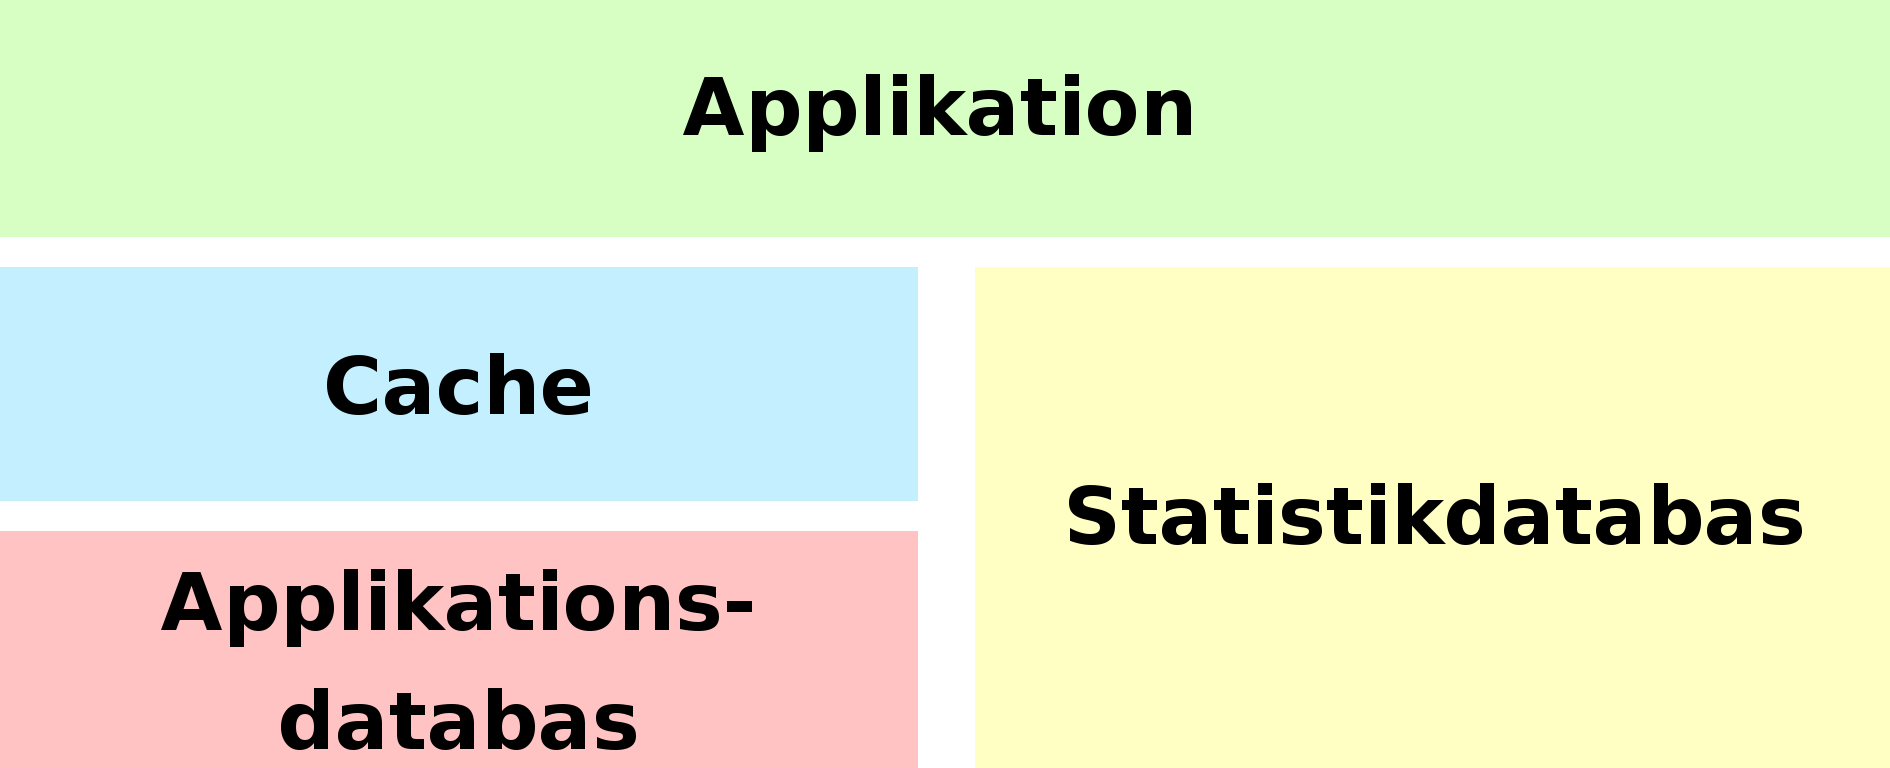
\includegraphics[width=120mm]{assets/images/smelementbackendparts.png}
\caption{Delarna av serverkomponenten}
\label{abstractbackend}
\end{figure}

Back-end systemet eller serverkomponeneten i SmartElement är den centrala delen av systemet var all data lagras och all filtrering sker. Systemet har i två gränssnitt, ett öppet som används av tagen för att hämta innehåll vid sidvisningar och ett stängt som används av en frontend vid konfiguration av sidor.

Hela back-end systemet är designat med en fokus på att vara "tillståndslöst" vad gäller hanteringen av förfrågnignar. I praktiken betyder detta att man inte skall behöva en session med back-enden för att kunna genomföra förfrågningar utan all information som behövs förses antingen i förfrågan, eller så kan den generaras från databasen. Detta betyder att t.ex. autentikationen är baserad på en nyckel som används för att generara en signatur för varje förfrågan. Orsaken till detta ligger i att det är lättare att skala systemet horisontellt, genom att lägga till applikationsservrar, då sessioner inte behöver synkroniseras mellan de olika servrarna.

Tekniskt sett så finns det fyra huvudsakliga komponenter i back-end systemet som kan skiljas åt, applikationen, caching-lagret, applikations-databasen och statistik-databasen. Denna uppdelning är gjord för att försöka tillåta för oberoende horisontell skalning av resurserna för de olika ansvarsområdena genom att lägga till eller ta bort instanser av de olika komponenterna i takt med behov.

\subsection{Komponenter}

\subsubsection{Matcher}

Den centrala delen av hanteringen av en sidvisning sker i den så kallade matchern som tar emot information om besökaren och söker fram det innehåll som skall skickas tillbaka. Rent tekniskt så tar matchern besökarobjektet, synkroniserar statistikdatabasen med besökarobjektet, söker fram sidobjektet ur cachinglagret (alternativt bygger det från databasen), använder sidobjektet för att generera det innehåll som skall sändas tillbaka och formaterar ett svar som skickas tillbaka till klienten.

\subsubsection{Besökarobjektet}

Besökarobjektet representerar en besökare på webbsidan och innehåller all information som systemet kunnat samla ihop. Besökarobjektet är det enda objekt i filtreringsprocessen som är designat att röra databasen.

När en förfrågan kommer in, kallas en factory metod som försöker hitta besökaren i statistikdatabasen. Om ett resultat hittas, uppdaterar factory metoden det befintliga objektet med den nya informationen från fårfrågningen. Om besökaren inte är igenkännd så skapas ett nytt besökarobjekt med den försedda informationen.

\subsubsection{Site ojektet}

% Graphic for TeX using PGF
% Title: /home/enberg/Diagram1.dia
% Creator: Dia v0.97.2
% CreationDate: Mon Apr 28 21:21:06 2014
% For: enberg
% \usepackage{tikz}
% The following commands are not supported in PSTricks at present
% We define them conditionally, so when they are implemented,
% this pgf file will use them.
\ifx\du\undefined
  \newlength{\du}
\fi
\setlength{\du}{15\unitlength}
\begin{tikzpicture}
\pgftransformxscale{1.000000}
\pgftransformyscale{-1.000000}
\definecolor{dialinecolor}{rgb}{0.000000, 0.000000, 0.000000}
\pgfsetstrokecolor{dialinecolor}
\definecolor{dialinecolor}{rgb}{1.000000, 1.000000, 1.000000}
\pgfsetfillcolor{dialinecolor}
\pgfsetlinewidth{0.100000\du}
\pgfsetdash{}{0pt}
\definecolor{dialinecolor}{rgb}{1.000000, 1.000000, 1.000000}
\pgfsetfillcolor{dialinecolor}
\fill (15.300000\du,-6.800000\du)--(15.300000\du,-5.400000\du)--(31.970000\du,-5.400000\du)--(31.970000\du,-6.800000\du)--cycle;
\definecolor{dialinecolor}{rgb}{0.000000, 0.000000, 0.000000}
\pgfsetstrokecolor{dialinecolor}
\draw (15.300000\du,-6.800000\du)--(15.300000\du,-5.400000\du)--(31.970000\du,-5.400000\du)--(31.970000\du,-6.800000\du)--cycle;
% setfont left to latex
\definecolor{dialinecolor}{rgb}{0.000000, 0.000000, 0.000000}
\pgfsetstrokecolor{dialinecolor}
\node at (23.635000\du,-5.850000\du){Site};
\definecolor{dialinecolor}{rgb}{1.000000, 1.000000, 1.000000}
\pgfsetfillcolor{dialinecolor}
\fill (15.300000\du,-5.400000\du)--(15.300000\du,-3.600000\du)--(31.970000\du,-3.600000\du)--(31.970000\du,-5.400000\du)--cycle;
\definecolor{dialinecolor}{rgb}{0.000000, 0.000000, 0.000000}
\pgfsetstrokecolor{dialinecolor}
\draw (15.300000\du,-5.400000\du)--(15.300000\du,-3.600000\du)--(31.970000\du,-3.600000\du)--(31.970000\du,-5.400000\du)--cycle;
% setfont left to latex
\definecolor{dialinecolor}{rgb}{0.000000, 0.000000, 0.000000}
\pgfsetstrokecolor{dialinecolor}
\node[anchor=west] at (15.450000\du,-4.700000\du){-elements};
% setfont left to latex
\definecolor{dialinecolor}{rgb}{0.000000, 0.000000, 0.000000}
\pgfsetstrokecolor{dialinecolor}
\node[anchor=west] at (15.450000\du,-3.900000\du){-customer};
\definecolor{dialinecolor}{rgb}{1.000000, 1.000000, 1.000000}
\pgfsetfillcolor{dialinecolor}
\fill (15.300000\du,-3.600000\du)--(15.300000\du,-2.600000\du)--(31.970000\du,-2.600000\du)--(31.970000\du,-3.600000\du)--cycle;
\definecolor{dialinecolor}{rgb}{0.000000, 0.000000, 0.000000}
\pgfsetstrokecolor{dialinecolor}
\draw (15.300000\du,-3.600000\du)--(15.300000\du,-2.600000\du)--(31.970000\du,-2.600000\du)--(31.970000\du,-3.600000\du)--cycle;
% setfont left to latex
\definecolor{dialinecolor}{rgb}{0.000000, 0.000000, 0.000000}
\pgfsetstrokecolor{dialinecolor}
\node[anchor=west] at (15.450000\du,-2.900000\du){+getContentFor(visitor:Visitor,elementIds)};
\end{tikzpicture}


Sidobjektet är det högsta objektet i hierarkin, det beskriver användarens webbplats i sin helhet. Från sidobjektet går alla relationer enda ner till filtren som används för att välja ut innehåll.

När matchern samlar ihop data för att skicka tillbaka till klienten så kallar den på siteobjektet med ett besökarobjekt och därefter sköter siteobjektet om att kalla på de olika elementen som sparats under sidan och ber dessa filtrera ut lämpligt innehåll innan det lämnar tillbaka kontroller till matchern.

Objektet är designat så att det kan kompileras till en entitet som går att spara i ett caching-lager för kunna hålla objekten i minne vid operation. Detta tillåter snabb åtkomst till data under en sidvisning och sparar på databasförfrågningar.

\subsubsection{Element objekten}

% Graphic for TeX using PGF
% Title: /home/enberg/Diagram2.dia
% Creator: Dia v0.97.2
% CreationDate: Mon Apr 28 21:24:10 2014
% For: enberg
% \usepackage{tikz}
% The following commands are not supported in PSTricks at present
% We define them conditionally, so when they are implemented,
% this pgf file will use them.
\ifx\du\undefined
  \newlength{\du}
\fi
\setlength{\du}{15\unitlength}
\begin{tikzpicture}
\pgftransformxscale{1.000000}
\pgftransformyscale{-1.000000}
\definecolor{dialinecolor}{rgb}{0.000000, 0.000000, 0.000000}
\pgfsetstrokecolor{dialinecolor}
\definecolor{dialinecolor}{rgb}{1.000000, 1.000000, 1.000000}
\pgfsetfillcolor{dialinecolor}
\pgfsetlinewidth{0.100000\du}
\pgfsetdash{}{0pt}
\definecolor{dialinecolor}{rgb}{1.000000, 1.000000, 1.000000}
\pgfsetfillcolor{dialinecolor}
\fill (6.100000\du,11.450000\du)--(6.100000\du,12.850000\du)--(14.300000\du,12.850000\du)--(14.300000\du,11.450000\du)--cycle;
\definecolor{dialinecolor}{rgb}{0.000000, 0.000000, 0.000000}
\pgfsetstrokecolor{dialinecolor}
\draw (6.100000\du,11.450000\du)--(6.100000\du,12.850000\du)--(14.300000\du,12.850000\du)--(14.300000\du,11.450000\du)--cycle;
% setfont left to latex
\definecolor{dialinecolor}{rgb}{0.000000, 0.000000, 0.000000}
\pgfsetstrokecolor{dialinecolor}
\node at (10.200000\du,12.400000\du){Element};
\definecolor{dialinecolor}{rgb}{1.000000, 1.000000, 1.000000}
\pgfsetfillcolor{dialinecolor}
\fill (6.100000\du,12.850000\du)--(6.100000\du,14.650000\du)--(14.300000\du,14.650000\du)--(14.300000\du,12.850000\du)--cycle;
\definecolor{dialinecolor}{rgb}{0.000000, 0.000000, 0.000000}
\pgfsetstrokecolor{dialinecolor}
\draw (6.100000\du,12.850000\du)--(6.100000\du,14.650000\du)--(14.300000\du,14.650000\du)--(14.300000\du,12.850000\du)--cycle;
% setfont left to latex
\definecolor{dialinecolor}{rgb}{0.000000, 0.000000, 0.000000}
\pgfsetstrokecolor{dialinecolor}
\node[anchor=west] at (6.250000\du,13.550000\du){-filterSets};
% setfont left to latex
\definecolor{dialinecolor}{rgb}{0.000000, 0.000000, 0.000000}
\pgfsetstrokecolor{dialinecolor}
\node[anchor=west] at (6.250000\du,14.350000\du){-contents};
\definecolor{dialinecolor}{rgb}{1.000000, 1.000000, 1.000000}
\pgfsetfillcolor{dialinecolor}
\fill (6.100000\du,14.650000\du)--(6.100000\du,15.650000\du)--(14.300000\du,15.650000\du)--(14.300000\du,14.650000\du)--cycle;
\definecolor{dialinecolor}{rgb}{0.000000, 0.000000, 0.000000}
\pgfsetstrokecolor{dialinecolor}
\draw (6.100000\du,14.650000\du)--(6.100000\du,15.650000\du)--(14.300000\du,15.650000\du)--(14.300000\du,14.650000\du)--cycle;
% setfont left to latex
\definecolor{dialinecolor}{rgb}{0.000000, 0.000000, 0.000000}
\pgfsetstrokecolor{dialinecolor}
\node[anchor=west] at (6.250000\du,15.350000\du){+contentFor(visitor)};
\end{tikzpicture}


Element objekten motsvarar ett HTML element på användarens webbplats, men de är ej bundna till någon specifik url eller sida på webbplatsen. Detta betyder att man kan använda samma element på olika sidor under samma webbplats om man vill, t.ex. i en side-bar eller som del av en navigation.

\subsubsection{FilterSet objekten}

% Graphic for TeX using PGF
% Title: /home/enberg/Documents/Thesis/assets/uml/Diagram3.dia
% Creator: Dia v0.97.2
% CreationDate: Mon Apr 28 21:27:22 2014
% For: enberg
% \usepackage{tikz}
% The following commands are not supported in PSTricks at present
% We define them conditionally, so when they are implemented,
% this pgf file will use them.
\ifx\du\undefined
  \newlength{\du}
\fi
\setlength{\du}{15\unitlength}
\begin{tikzpicture}
\pgftransformxscale{1.000000}
\pgftransformyscale{-1.000000}
\definecolor{dialinecolor}{rgb}{0.000000, 0.000000, 0.000000}
\pgfsetstrokecolor{dialinecolor}
\definecolor{dialinecolor}{rgb}{1.000000, 1.000000, 1.000000}
\pgfsetfillcolor{dialinecolor}
\pgfsetlinewidth{0.100000\du}
\pgfsetdash{}{0pt}
\definecolor{dialinecolor}{rgb}{1.000000, 1.000000, 1.000000}
\pgfsetfillcolor{dialinecolor}
\fill (11.850000\du,9.700000\du)--(11.850000\du,11.100000\du)--(18.895000\du,11.100000\du)--(18.895000\du,9.700000\du)--cycle;
\definecolor{dialinecolor}{rgb}{0.000000, 0.000000, 0.000000}
\pgfsetstrokecolor{dialinecolor}
\draw (11.850000\du,9.700000\du)--(11.850000\du,11.100000\du)--(18.895000\du,11.100000\du)--(18.895000\du,9.700000\du)--cycle;
% setfont left to latex
\definecolor{dialinecolor}{rgb}{0.000000, 0.000000, 0.000000}
\pgfsetstrokecolor{dialinecolor}
\node at (15.372500\du,10.650000\du){FilterSet};
\definecolor{dialinecolor}{rgb}{1.000000, 1.000000, 1.000000}
\pgfsetfillcolor{dialinecolor}
\fill (11.850000\du,11.100000\du)--(11.850000\du,12.100000\du)--(18.895000\du,12.100000\du)--(18.895000\du,11.100000\du)--cycle;
\definecolor{dialinecolor}{rgb}{0.000000, 0.000000, 0.000000}
\pgfsetstrokecolor{dialinecolor}
\draw (11.850000\du,11.100000\du)--(11.850000\du,12.100000\du)--(18.895000\du,12.100000\du)--(18.895000\du,11.100000\du)--cycle;
% setfont left to latex
\definecolor{dialinecolor}{rgb}{0.000000, 0.000000, 0.000000}
\pgfsetstrokecolor{dialinecolor}
\node[anchor=west] at (12.000000\du,11.800000\du){-filters};
\definecolor{dialinecolor}{rgb}{1.000000, 1.000000, 1.000000}
\pgfsetfillcolor{dialinecolor}
\fill (11.850000\du,12.100000\du)--(11.850000\du,13.100000\du)--(18.895000\du,13.100000\du)--(18.895000\du,12.100000\du)--cycle;
\definecolor{dialinecolor}{rgb}{0.000000, 0.000000, 0.000000}
\pgfsetstrokecolor{dialinecolor}
\draw (11.850000\du,12.100000\du)--(11.850000\du,13.100000\du)--(18.895000\du,13.100000\du)--(18.895000\du,12.100000\du)--cycle;
% setfont left to latex
\definecolor{dialinecolor}{rgb}{0.000000, 0.000000, 0.000000}
\pgfsetstrokecolor{dialinecolor}
\node[anchor=west] at (12.000000\du,12.800000\du){+matches(visitor)};
\end{tikzpicture}


Ett element inehåller filterset, innehåll och ett status. Filterseten är samlingar av filter med en länk till ett innehållsobjekt samt en prioritet inom elementet. När sidobjektet kallar på ett element för att få tillbaka det passliga innehållet kör elementet igenom sin samling filter set och ser om de matchar besökarobjektet. Om fler en ett filterset matchar så väljs det med högsta prioritet. När ett filterset valts ut så returnerar elementet det innehåll som filtersetet är länkat till, om inget filterset matchar så returneras ett tomt resultat.

Filterseten bygger tillsammans med filtren på en design princip som kallas för "Strategy pattern", var idén är att man genoma att definiera ett bra gränsnitt för en process, lämnar systemet öppet för enkel vidareutveckling i ett senare skede. FilterSet objektet i samband med Besökar objektet utgör tillsammans det kontext i vlilket strategierna (Filtren) appliceras.

\subsubsection{Filter objekten}

% Graphic for TeX using PGF
% Title: /home/enberg/Diagram4.dia
% Creator: Dia v0.97.2
% CreationDate: Mon Apr 28 21:29:10 2014
% For: enberg
% \usepackage{tikz}
% The following commands are not supported in PSTricks at present
% We define them conditionally, so when they are implemented,
% this pgf file will use them.
\ifx\du\undefined
  \newlength{\du}
\fi
\setlength{\du}{15\unitlength}
\begin{tikzpicture}
\pgftransformxscale{1.000000}
\pgftransformyscale{-1.000000}
\definecolor{dialinecolor}{rgb}{0.000000, 0.000000, 0.000000}
\pgfsetstrokecolor{dialinecolor}
\definecolor{dialinecolor}{rgb}{1.000000, 1.000000, 1.000000}
\pgfsetfillcolor{dialinecolor}
\pgfsetlinewidth{0.100000\du}
\pgfsetdash{}{0pt}
\definecolor{dialinecolor}{rgb}{1.000000, 1.000000, 1.000000}
\pgfsetfillcolor{dialinecolor}
\fill (17.500000\du,11.450000\du)--(17.500000\du,12.850000\du)--(24.545000\du,12.850000\du)--(24.545000\du,11.450000\du)--cycle;
\definecolor{dialinecolor}{rgb}{0.000000, 0.000000, 0.000000}
\pgfsetstrokecolor{dialinecolor}
\draw (17.500000\du,11.450000\du)--(17.500000\du,12.850000\du)--(24.545000\du,12.850000\du)--(24.545000\du,11.450000\du)--cycle;
% setfont left to latex
\definecolor{dialinecolor}{rgb}{0.000000, 0.000000, 0.000000}
\pgfsetstrokecolor{dialinecolor}
\node at (21.022500\du,12.400000\du){Filter};
\definecolor{dialinecolor}{rgb}{1.000000, 1.000000, 1.000000}
\pgfsetfillcolor{dialinecolor}
\fill (17.500000\du,12.850000\du)--(17.500000\du,15.450000\du)--(24.545000\du,15.450000\du)--(24.545000\du,12.850000\du)--cycle;
\definecolor{dialinecolor}{rgb}{0.000000, 0.000000, 0.000000}
\pgfsetstrokecolor{dialinecolor}
\draw (17.500000\du,12.850000\du)--(17.500000\du,15.450000\du)--(24.545000\du,15.450000\du)--(24.545000\du,12.850000\du)--cycle;
% setfont left to latex
\definecolor{dialinecolor}{rgb}{0.000000, 0.000000, 0.000000}
\pgfsetstrokecolor{dialinecolor}
\node[anchor=west] at (17.650000\du,13.550000\du){-type};
% setfont left to latex
\definecolor{dialinecolor}{rgb}{0.000000, 0.000000, 0.000000}
\pgfsetstrokecolor{dialinecolor}
\node[anchor=west] at (17.650000\du,14.350000\du){-filtersOn};
% setfont left to latex
\definecolor{dialinecolor}{rgb}{0.000000, 0.000000, 0.000000}
\pgfsetstrokecolor{dialinecolor}
\node[anchor=west] at (17.650000\du,15.150000\du){-filterValue};
\definecolor{dialinecolor}{rgb}{1.000000, 1.000000, 1.000000}
\pgfsetfillcolor{dialinecolor}
\fill (17.500000\du,15.450000\du)--(17.500000\du,16.450000\du)--(24.545000\du,16.450000\du)--(24.545000\du,15.450000\du)--cycle;
\definecolor{dialinecolor}{rgb}{0.000000, 0.000000, 0.000000}
\pgfsetstrokecolor{dialinecolor}
\draw (17.500000\du,15.450000\du)--(17.500000\du,16.450000\du)--(24.545000\du,16.450000\du)--(24.545000\du,15.450000\du)--cycle;
% setfont left to latex
\definecolor{dialinecolor}{rgb}{0.000000, 0.000000, 0.000000}
\pgfsetstrokecolor{dialinecolor}
\node[anchor=west] at (17.650000\du,16.150000\du){+matches(visitor)};
\end{tikzpicture}


Filterobjekten är i slutendan de objekt som utför test mot besökarobjektet. De består av en filtertyp som definierar hur de jämför data, ett fältid som de använder för att läsa ut data ur besökarobjektet, ett värde som de testar mot och ett villkor som de använder för att utföra testet.

Filterobjekten implementerar strategin i filtreringen som utförs i sammband med filterseten. Filter tar endast ställning till en sak och returnerar ett booleanskt värde beroende på om kriteriet möts eller ej. Filtersetet vet endast att det kan ställa frågan av godtyckligt filter och filtret i sig vet att frågan alltid kommer att ställas på samma vis med likadan input.

\subsubsection{Content objekten}

% Graphic for TeX using PGF
% Title: /home/enberg/Diagram5.dia
% Creator: Dia v0.97.2
% CreationDate: Mon Apr 28 21:31:26 2014
% For: enberg
% \usepackage{tikz}
% The following commands are not supported in PSTricks at present
% We define them conditionally, so when they are implemented,
% this pgf file will use them.
\ifx\du\undefined
  \newlength{\du}
\fi
\setlength{\du}{15\unitlength}
\begin{tikzpicture}
\pgftransformxscale{1.000000}
\pgftransformyscale{-1.000000}
\definecolor{dialinecolor}{rgb}{0.000000, 0.000000, 0.000000}
\pgfsetstrokecolor{dialinecolor}
\definecolor{dialinecolor}{rgb}{1.000000, 1.000000, 1.000000}
\pgfsetfillcolor{dialinecolor}
\pgfsetlinewidth{0.100000\du}
\pgfsetdash{}{0pt}
\definecolor{dialinecolor}{rgb}{1.000000, 1.000000, 1.000000}
\pgfsetfillcolor{dialinecolor}
\fill (12.250000\du,13.250000\du)--(12.250000\du,14.650000\du)--(16.335000\du,14.650000\du)--(16.335000\du,13.250000\du)--cycle;
\definecolor{dialinecolor}{rgb}{0.000000, 0.000000, 0.000000}
\pgfsetstrokecolor{dialinecolor}
\draw (12.250000\du,13.250000\du)--(12.250000\du,14.650000\du)--(16.335000\du,14.650000\du)--(16.335000\du,13.250000\du)--cycle;
% setfont left to latex
\definecolor{dialinecolor}{rgb}{0.000000, 0.000000, 0.000000}
\pgfsetstrokecolor{dialinecolor}
\node at (14.292500\du,14.200000\du){Content};
\definecolor{dialinecolor}{rgb}{1.000000, 1.000000, 1.000000}
\pgfsetfillcolor{dialinecolor}
\fill (12.250000\du,14.650000\du)--(12.250000\du,17.250000\du)--(16.335000\du,17.250000\du)--(16.335000\du,14.650000\du)--cycle;
\definecolor{dialinecolor}{rgb}{0.000000, 0.000000, 0.000000}
\pgfsetstrokecolor{dialinecolor}
\draw (12.250000\du,14.650000\du)--(12.250000\du,17.250000\du)--(16.335000\du,17.250000\du)--(16.335000\du,14.650000\du)--cycle;
% setfont left to latex
\definecolor{dialinecolor}{rgb}{0.000000, 0.000000, 0.000000}
\pgfsetstrokecolor{dialinecolor}
\node[anchor=west] at (12.400000\du,15.350000\du){-name};
% setfont left to latex
\definecolor{dialinecolor}{rgb}{0.000000, 0.000000, 0.000000}
\pgfsetstrokecolor{dialinecolor}
\node[anchor=west] at (12.400000\du,16.150000\du){-type};
% setfont left to latex
\definecolor{dialinecolor}{rgb}{0.000000, 0.000000, 0.000000}
\pgfsetstrokecolor{dialinecolor}
\node[anchor=west] at (12.400000\du,16.950000\du){-data};
\end{tikzpicture}


Content objektet är den data som returneras till klienten efter att filtreringen skett. Systemet sätter ingen restriktion på datan annan än att det måste kunna sparas som en textsträng. Detta betyder att man kan producera avancerad funktionalitet genom att t.ex. spara javascript-kod eller json-data som innehåll och på så vis använda SmartElement för att styra exekvering på klienten. Det betyder också att systemet inte sätter så stora krav på den kallaren eftersom det enda som är viktigt är att klienten kan tolka datan som returneras, detta betyder att man i princip kunde skapa godtycklig klient till backenden genom att implementera protokollet som tagen använder.

\subsection{Javascript tagen}

Javascript tagen är en kort kod som laddas i samband med sidan och samlar ihop informaiton om användaren och sedan skickar denna information till back-end sytemet för processering.

Tagen börjar med att skapa en kaka på klienten om ingen redan existerar, skapar det besökar id som genom systemet används för att identifiera besökaren, registrerar tiden för sidvisningen, beräknar besökets längd, samlar ihop data om besökaren och sänder den till back-enden.

Efter att back-enden processerat förfrågan och returnerat data för de element som begärts så är standardbeteendet att backenden genom ett JSONP-svar kallar på tagen som uppdaterar dokumentet med det returnerade innehållet. Vilken funktion som kallas kan dock ändras och man kan genom att specifcera en callback ändra på funktionskallet i JSONP-svaret och på så vis använda egen logik för uppdateringen av innehållet.

\subsection{Begränsningar}

Systemet utvecklades med relativt låg budget och därigenom en del begränsningar på tekniken och hårdvaran som fanns tillgänglig. Detta återspeglar sig i en del begränsningar i själva systemet samt i funktionalitet som inte implementerats.



% vim: set tw=78:ts=2:sw=2:et:fdm=marker:wrap:wm=78:ft=tex
% vim: spell spelllang=sv
